\documentclass[12pt,a4paper]{report}

\usepackage[left=1.5in,right=1in,top=1in,bottom=1in]{geometry}
\usepackage{graphicx}
\usepackage{amsmath,amssymb}
\usepackage{array}
\usepackage{booktabs}
\usepackage{longtable}
\usepackage{setspace}
\usepackage{url}
\usepackage{cite}

\graphicspath{{assets/}}

\onehalfspacing
\renewcommand{\arraystretch}{1.2}

\begin{document}

% =========================================================
% TITLE PAGE
% =========================================================

\begin{titlepage}

% \begin{center}
% \begin{tabular}{@{}>{\centering\arraybackslash}m{0.27\textwidth}
%                     >{\centering\arraybackslash}m{0.68\textwidth}@{}}

% \IfFileExists{assets/SNU-logo.png}
% {\includegraphics[width=4cm]{assets/SNU-logo.png}}
% {\fbox{\parbox[c][2cm][c]{3.5cm}{\centering SNU-logo.png}}}

% &

% \begin{minipage}{\linewidth}
\centering
{\large \textbf{Shiv Nadar University-Chennai}}\\[0.1cm]
{\normalsize Kalavakkam, Tamil Nadu - 603110, India}\\[0.1cm]
{\normalsize Website: \texttt{www.snuchennai.edu.in}}
% \end{minipage}

% \end{tabular}
% \end{center}

\vspace{0.2cm}
\hrule
% \vspace{1cm}

\begin{center}

{\large \textbf{Department of Computer Science and Engineering }}\\[1cm]

{\large \textbf{CAPSTONE PROJECT REPORT}}\\

{\large \textbf{Phase 1 - Review 3}}\\[1cm]


{\large \textbf{Tiny Object Detection in Aerial Images}}\\[1cm]

{\large \textbf{Submitted by}}\\[0.3cm]

\begin{tabular}{p{6cm}p{5cm}}
\toprule
\centering \textbf{Student Name} &
\centering \arraybackslash \textbf{Registration Number}\\
\midrule
\centering Anjana K &
\centering \arraybackslash 23011101022\\
\centering Lalith Adithyan S &
\centering \arraybackslash 23011101071\\
\bottomrule
\end{tabular}

\vfill


{\large \textbf{Under the guidance of}}\\[0.2cm]
{\large Dr.\ Chandrakala S}\\
Professor\\
\vspace{0.6cm}
% \begin{center}
\begin{tabular}{c}
Approved By: \\
 \\
 \\
\shortstack{\rule{4cm}{0.4pt}\\
Dr. Chandrakala S\\
Project Guide}
\end{tabular}

\vfill



\end{center}
\end{titlepage}

% =========================================================
% CERTIFICATE / REPORT BODY
% =========================================================

\pagenumbering{roman}
\setcounter{chapter}{2}


\chapter{Dataset / Simulation Details}
% which ever is suitable for your project
\section{Dataset or Simulation Environment}
The evaluation of the object detection models is conducted on two primary large-scale aerial benchmarks: the VisDrone2019 dataset~\cite{zhu2021visdrone,du2018visdrone} and the DOTA-v1.0 dataset~\cite{xia2018dota,ding2021dota}. These datasets were explicitly chosen due to their rigorous representation of real-world aerial perception challenges~\cite{yang2026uavdet}. UAV imagery is characterized by extreme scale variation, ranging from massive infrastructures to minute pedestrians, where small objects are easily overwhelmed by complex backgrounds. Furthermore, non-uniform object distributions and varying drone flight altitudes introduce severe spatial heterogeneity. In this project, the primary focus is directed toward detecting highly dense object clusters and camouflaged targets that naturally blend into their surrounding environments, making them exceptionally difficult to isolate from background noise.

\section{Dataset Description}
The project relies on two distinct aerial datasets to validate both low-altitude and high-altitude detection robustness against dense and visually obscured targets:

\subsection*{1. VisDrone2019 Dataset}
This dataset consists of images captured by various drone platforms across multiple urban and rural environments under different weather and lighting conditions. It comprises 6,471 training images, 548 validation images, and 1,610 testing images~\cite{zhu2021visdrone}. The dataset features 10 target categories: pedestrian, person, car, van, bus, truck, motor, bicycle, awning-tricycle, and tricycle~\cite{zhu2021visdrone,du2018visdrone}. 

\begin{figure}[htbp]
    \centering
    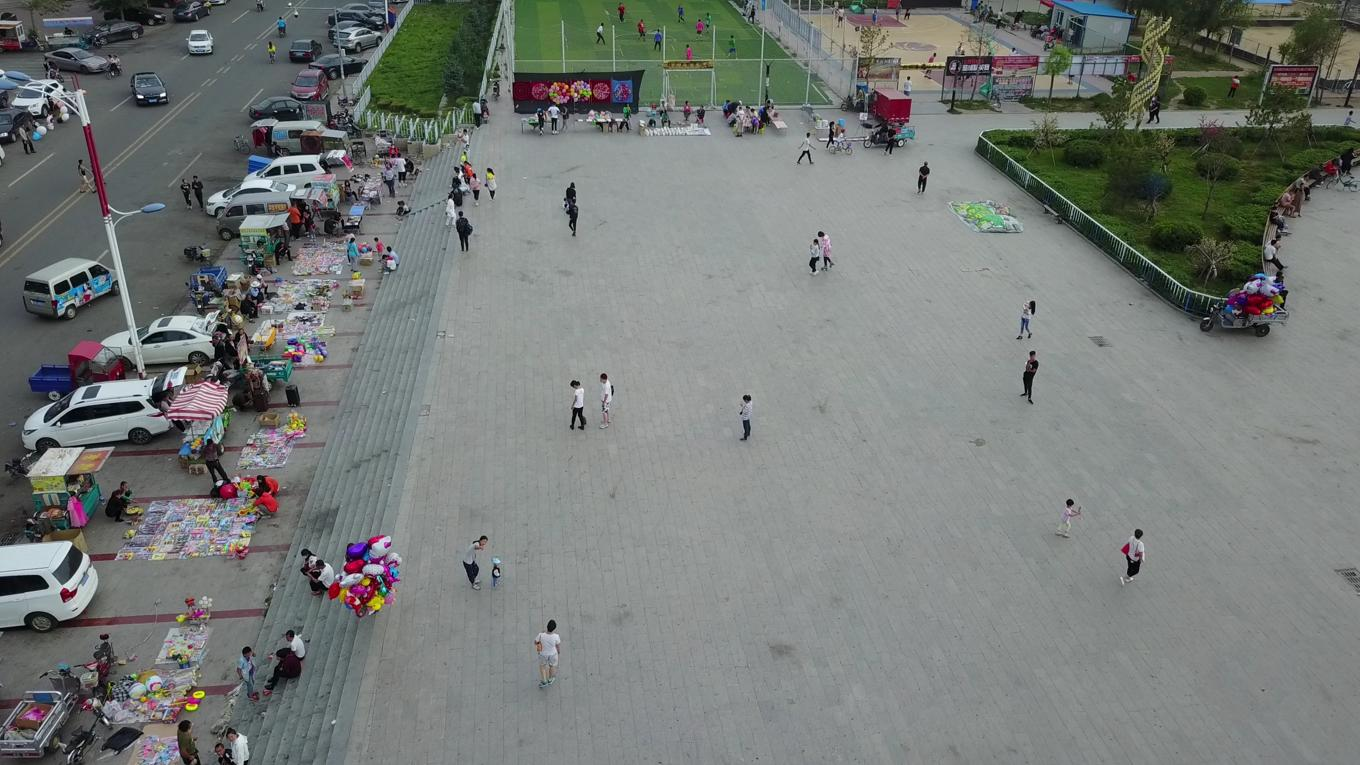
\includegraphics[width=0.8\textwidth]{assets/visdrone_sample.jpg}
    \caption{Sample images from the VisDrone2019 dataset showcasing high-density small objects in urban environments.}
    \label{fig:visdrone_sample}
\end{figure}

\begin{figure}[htbp]
    \centering
    \begin{tabular}{cc}
        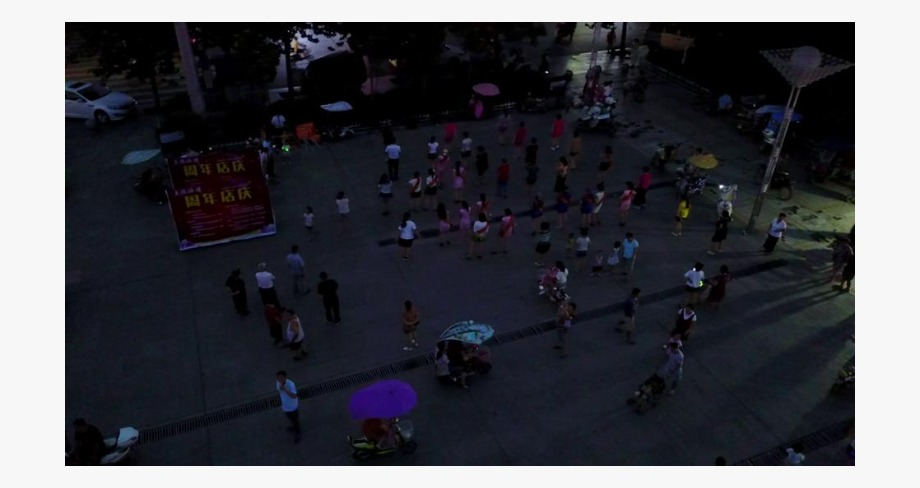
\includegraphics[width=0.48\textwidth]{assets/GT_VisDrone.jpeg} &
        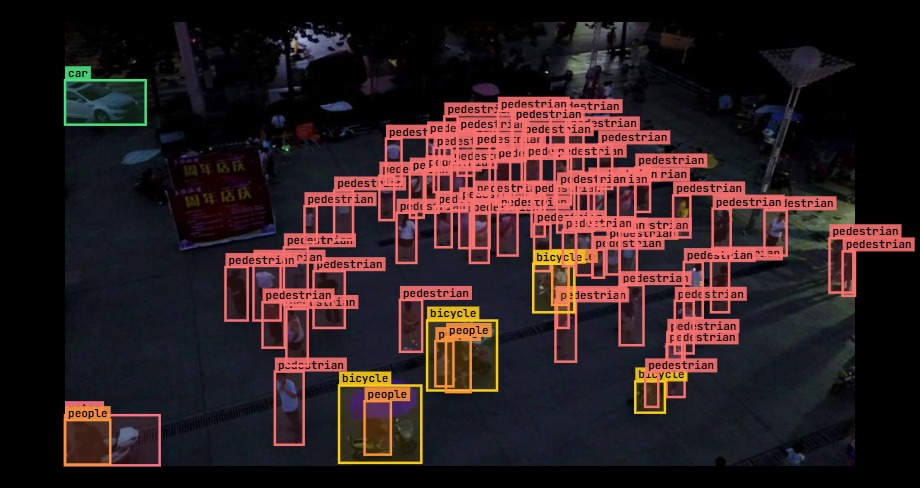
\includegraphics[width=0.48\textwidth]{assets/GT_annotated.jpeg} \\
        \small (a) Raw VisDrone aerial capture & \small (b) Ground Truth (GT) annotated bounding boxes
    \end{tabular}
    \caption{Visual comparison of a raw VisDrone aerial scene and its corresponding Ground Truth (GT) annotations, illustrating extreme crowd density, sub-16-pixel target dimensions, and severe target overlapping under low illumination.}
    \label{fig:visdrone_gt}
\end{figure}

\subsection*{2. DOTA-v1.0 Dataset}
DOTA-v1.0 is a large-scale dataset for object detection in aerial images, containing 2,806 images with spatial dimensions ranging from $800 \times 800$ to $4000 \times 4000$ pixels~\cite{xia2018dota}. It contains 188,282 annotated object instances across 15 categories: plane, ship, storage tank, baseball diamond, tennis court, basketball court, ground track field, harbor, bridge, large vehicle, small vehicle, helicopter, soccer ball field, roundabout, and swimming pool~\cite{xia2018dota,ding2021dota}.

\begin{figure}[htbp]
    \centering
    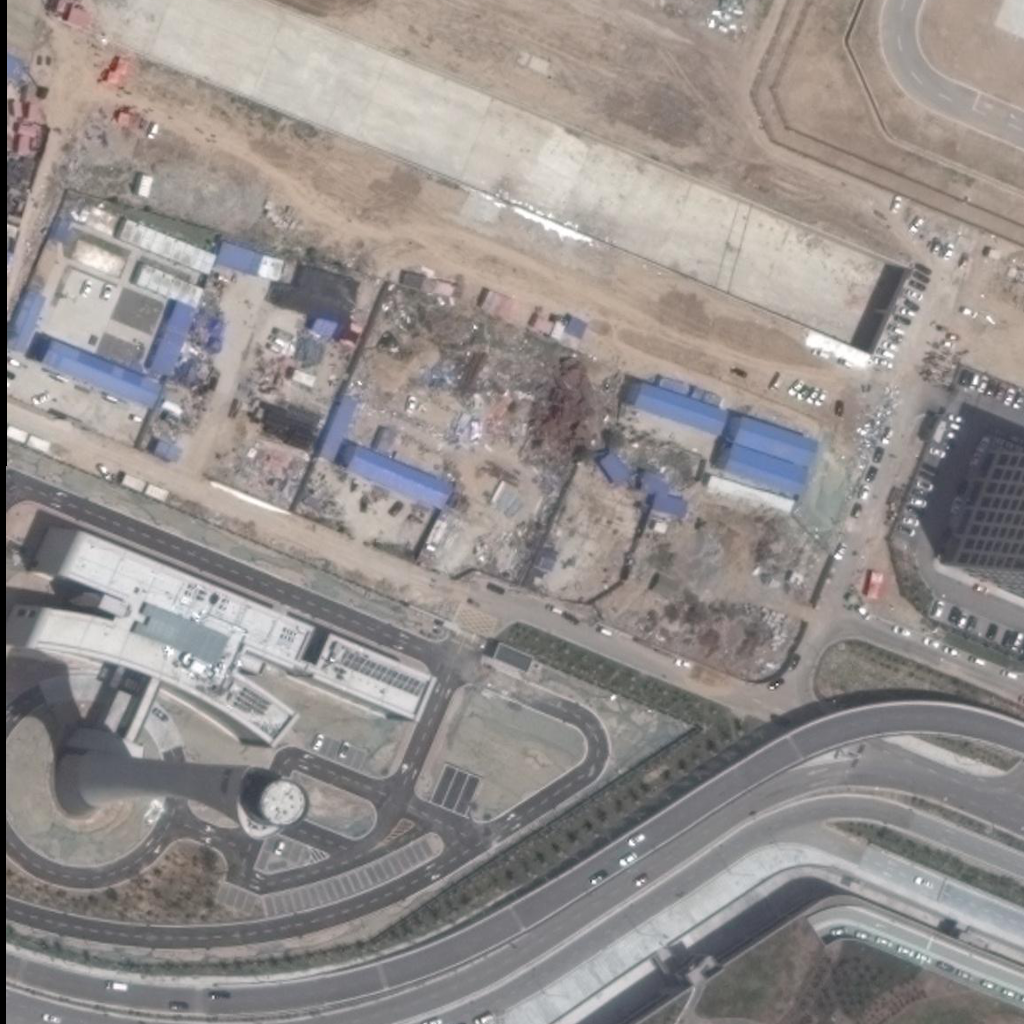
\includegraphics[width=0.8\textwidth]{assets/dota_sample.png}
    \caption{Sample aerial images from the DOTA-v1.0 dataset demonstrating extreme scale variations and arbitrary object orientations.}
    \label{fig:dota_sample}
\end{figure}

\section{Data Collection and Preprocessing}
Due to the massive resolution and varied formats of the source imagery, a rigorous preprocessing pipeline is applied before feeding the data into the detection network:
\begin{itemize}
    \item \textbf{Image Tiling and Cropping:} Because DOTA-v1.0 images can reach up to $4000 \times 4000$ pixels, feeding them directly into the network exceeds GPU memory limits. The source images are cropped into $1024 \times 1024$ patches with a 200-pixel overlap to ensure targets on the boundaries are not severed~\cite{xia2018dota,akyron2022sahi}. VisDrone images are resized to a standardized $640 \times 640$ resolution, with sliding-window patch inference applied to dense clusters~\cite{yang2019clustered}.
    \item \textbf{Spatio-Frequency Extraction:} To address the camouflage effect and textural confusion (e.g., ground litter resembling small vehicles), preprocessing includes the extraction of a Laplacian of Gaussian (LoG) cue ($\sigma \in \{1, 2, 4\}$)~\cite{lindeberg1994scale}. This process separates high-frequency structural edges from low-frequency background noise, creating a vital control signal that guides the network's multi-scale scanning.
    \item \textbf{Data Augmentation:} To prevent overfitting and improve the model's robustness against complex background clutter, several augmentation techniques are applied. These include Mosaic and MixUp to simulate heavily crowded scenes~\cite{bochkovskiy2020yolov4,zhang2018mixup}, alongside standard random flipping, random cropping, and HSV color space adjustments. 
\end{itemize}

\section{Dataset Characteristics}
The defining characteristics of both datasets are the extreme scale imbalance, dense occlusion, and the presence of objects that camouflage into the terrain. In aerial photography, small targets occupy only a few pixels and exhibit extremely low contrast against complex backgrounds, effectively blending them into their surroundings. For instance, in the VisDrone dataset, small objects (sub-32 pixels) dominate the overall target distribution, while large objects represent a very small fraction of the data~\cite{wang2021normalized,xu2021dot}, as visually substantiated by the dense ground truth annotations in Figure~\ref{fig:visdrone_gt}. 

\begin{figure}[htbp]
    \centering
    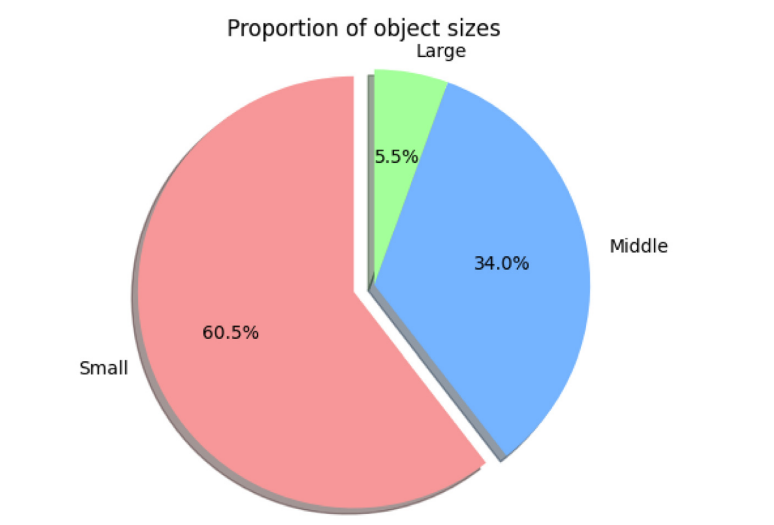
\includegraphics[width=0.7\textwidth]{assets/ObjectSizes.png}
    \caption{Proportion of small, medium, and large object instances, illustrating the heavy skew toward tiny targets in aerial imagery.}
    \label{fig:scale_distribution}
\end{figure}

\begin{figure}[htbp]
    \centering
    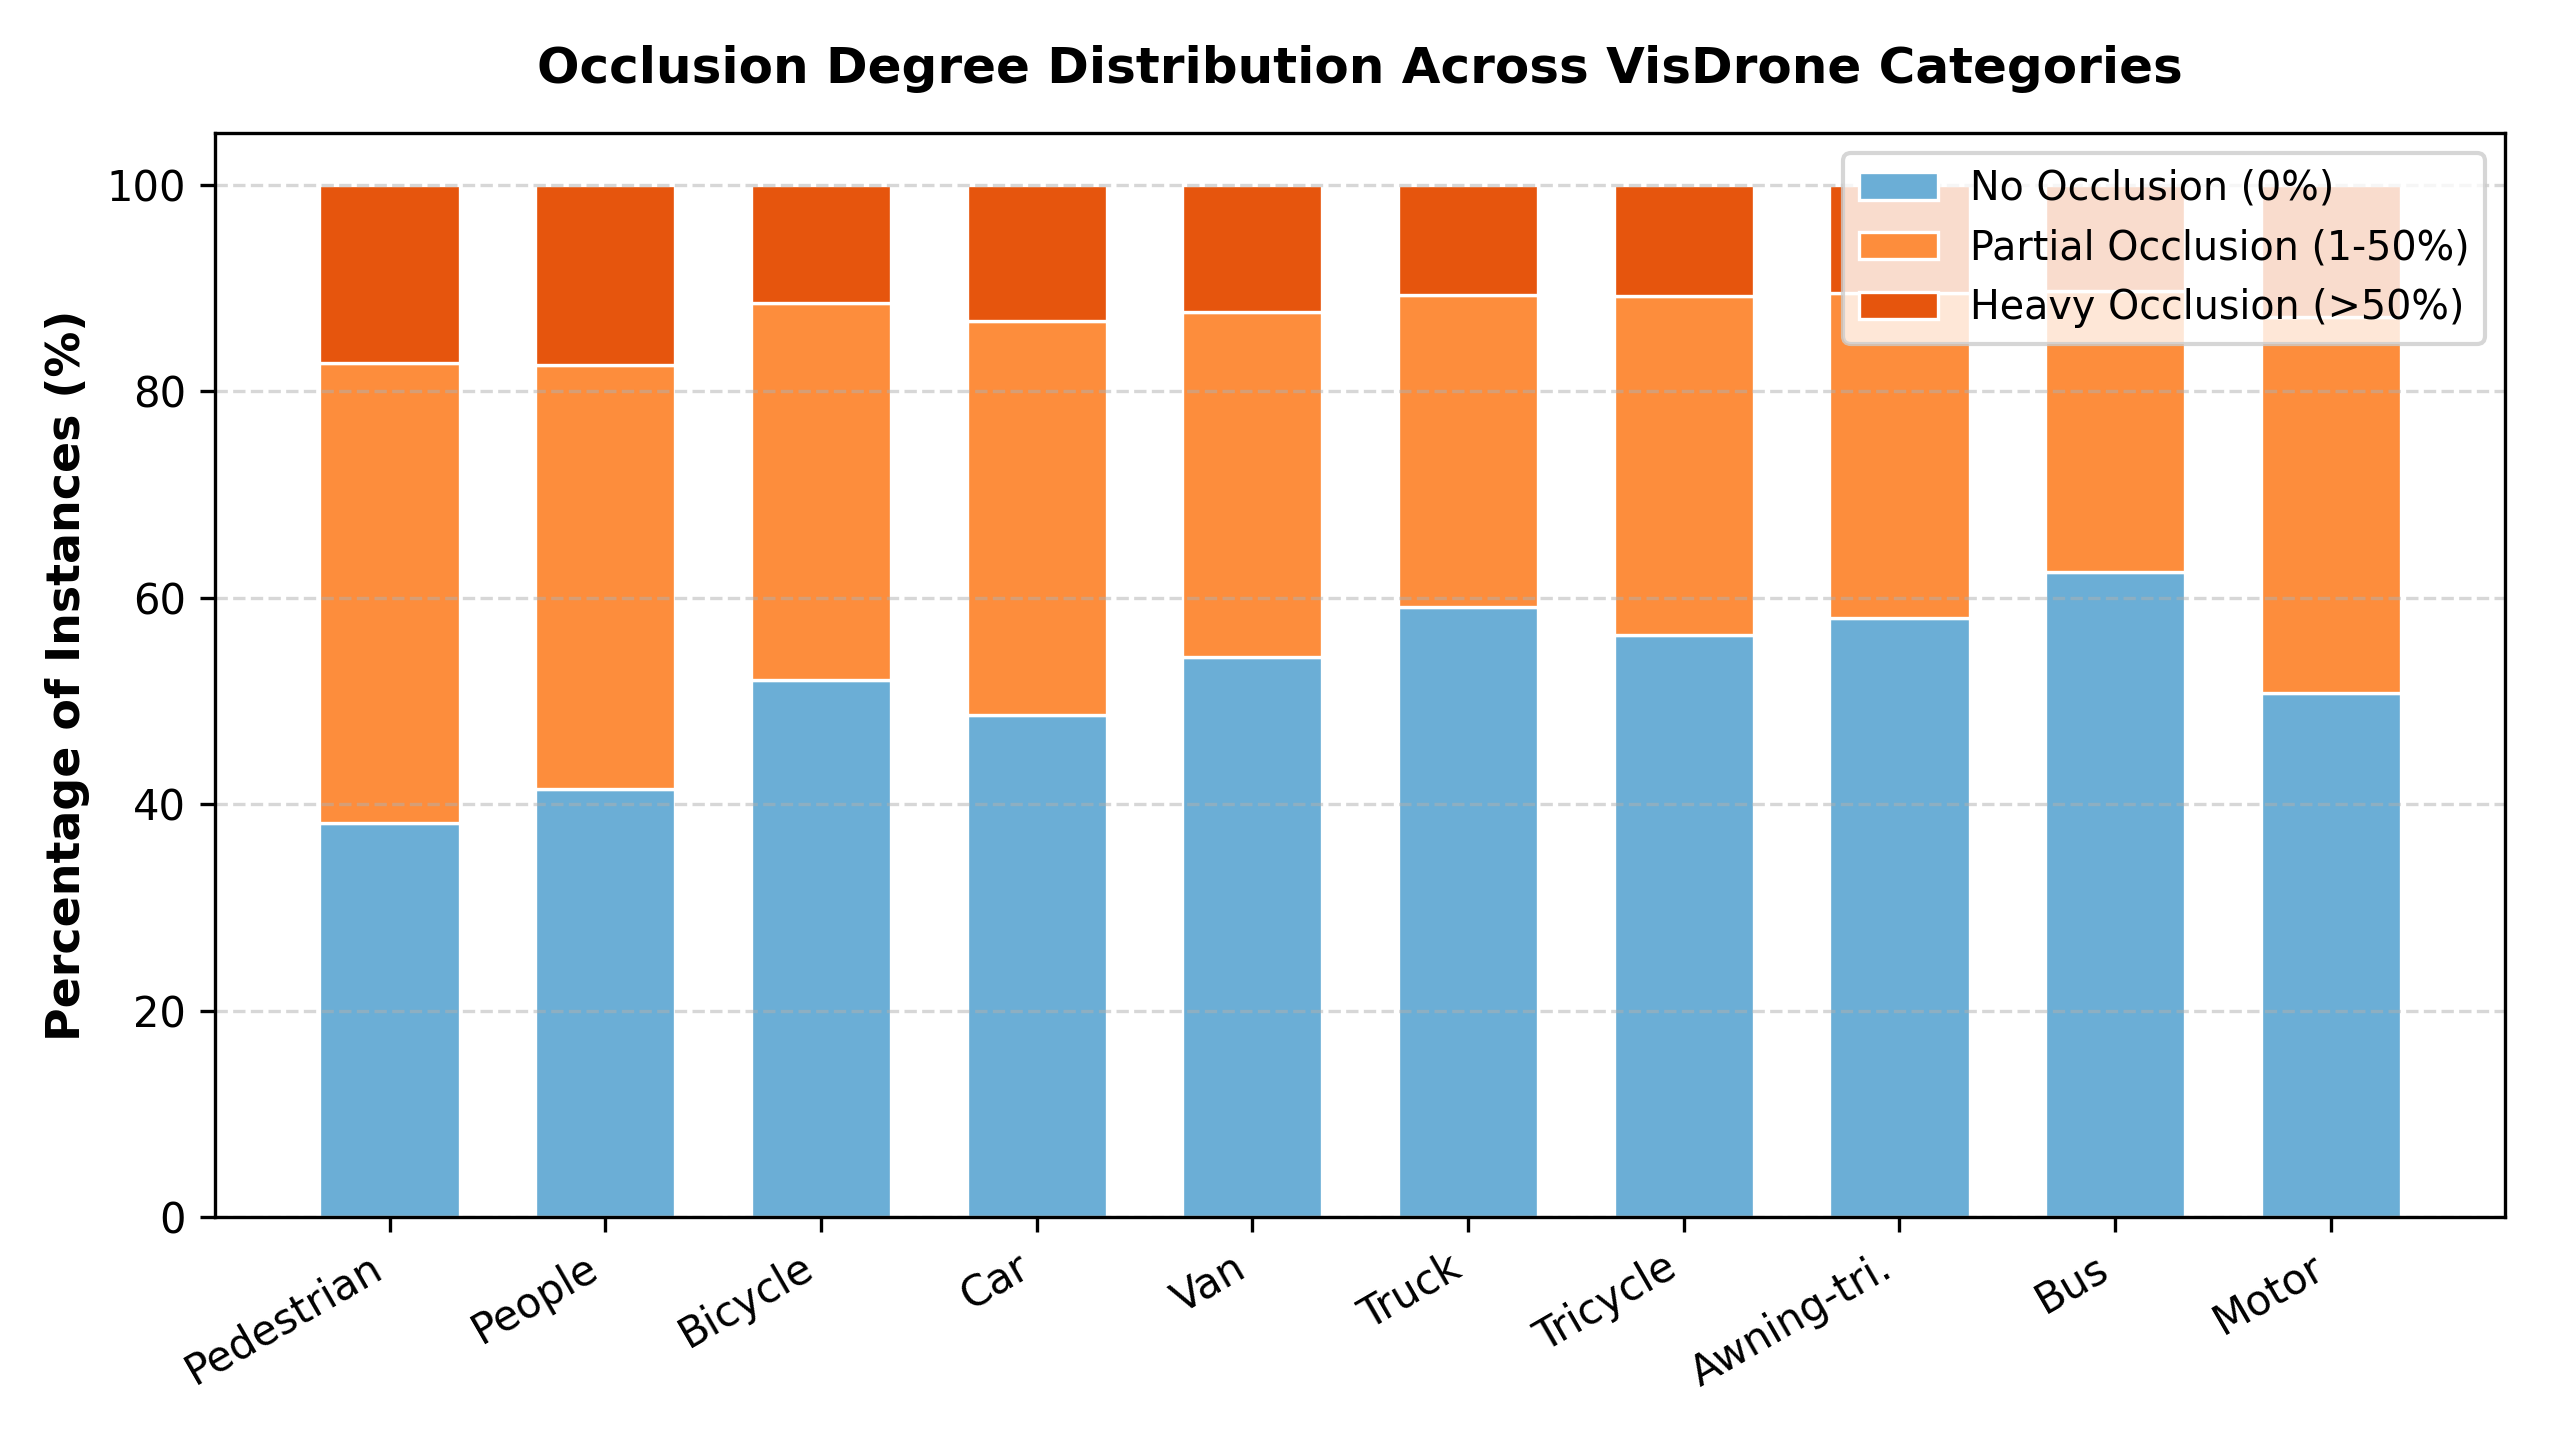
\includegraphics[width=0.75\textwidth]{assets/occlusion_chart.png}
    \caption{Occlusion degree distribution per category, highlighting the severe target overlapping present in drone-captured scenes.}
    \label{fig:occlusion_chart}
\end{figure}

\section{Assumptions and Limitations}
While preparing the datasets for model evaluation, several constraints and assumptions were acknowledged:
\begin{enumerate}
    \item \textbf{Optical Clarity Assumption:} The primary datasets assume relatively clear optical conditions. While varying illumination is present, severe atmospheric degradations (such as dense fog, heavy rain, or complete darkness) are underrepresented. Detecting highly camouflaged or super tiny objects in unseen haze remains a fundamental limitation without specialized domain adaptation.
    \item \textbf{Annotation Noise in Dense Clusters:} In ultra-dense scenes (e.g., massive crowds or congested parking lots), human annotation naturally introduces marginal localization errors or missed labels for highly occluded sub-16-pixel targets, which establishes a slight theoretical ceiling on supervised training precision.
    \item \textbf{Hardware Constraints:} It is assumed that raw high-resolution aerial images cannot be processed in a single forward pass during real-time edge deployment. The necessity of sliding-window cropping or resizing inherently risks losing the absolute widest macro-contextual cues needed to distinguish certain camouflaged objects from the background.
\end{enumerate}


\chapter{System Model}

\section{System Overview}
Aerial surveillance platforms frequently encounter severe visual ambiguity stemming from two intertwined perceptual challenges: \textbf{target camouflage} and \textbf{extreme multi-scale variance}. In real-world drone imagery, ground objects (such as light gray vehicles on faded concrete, dark trucks under canopy shadows, or camouflaged containers on textured dirt) exhibit near-zero spectral contrast against their surrounding terrain in RGB color space ($|\Delta I_{\text{RGB}}| \to 0$). Standard convolutional detectors and uniform Vision State-Space Models (Mamba)~\cite{gu2023mamba,liu2024vmamba} struggle because:
\begin{enumerate}
    \item \textbf{Deceit of Spatial RGB Pixels:} Color alone cannot distinguish real engineered objects from visual clutter such as painted road surfaces, trash mounds, or irregular roof fixtures.
    \item \textbf{The Receptive Field Dilemma in Atrous Convolution:} Standard atrous (dilated) convolution is typically applied with a static dilation rate $d$. When $d$ is kept small ($d=1$), the effective receptive field cannot capture contextual information required to disambiguate large, camouflaged structures. Conversely, when a high fixed dilation is used ($d \ge 3$), the kernel introduces severe \textit{gridding and checkerboard sampling artifacts}: minute objects ($4 \times 4$ to $12 \times 12$ pixels) fall entirely into the un-sampled gaps between kernel grid points, causing complete target loss.
    \item \textbf{Uncalibrated Sequence Modeling in Mamba:} Standard 1D selective scanning in Vision Mamba treats every patch equally, allowing immense expanses of background clutter ($>95\%$ of drone scenes) to saturate the recurrent hidden state $h_t$, attenuating the weak gradient signals of camouflaged objects.
\end{enumerate}

To overcome these foundational roadblocks, the proposed system introduces a dual-mechanism framework:
\begin{itemize}
    \item \textbf{Spatio-Frequency Laplacian of Gaussian (LoG) Perception:} Breaks target camouflage by decoupling high-frequency geometric boundary signatures from deceptive low-frequency surface textures, while concurrently extracting the intrinsic characteristic scale of each object.
    \item \textbf{Object-Scale-Modulated Adaptive Dilated Convolution (OS-ADC):} Modulates local atrous dilation rates ($d \in \{1, 2, 4\}$) and continuous deformable sampling offsets according to the derived object scale, feeding scale-calibrated tokens into the 1D selective Mamba backbone.
\end{itemize}

\section{Combating Camouflaged Objects via Spatio-Frequency LoG Perception}
While camouflaged targets intentionally mimic background color distributions, physical objects inevitably possess sharp material transitions, structural phase inflections, and rigid geometric contours. The system exploits this physical property through a multi-scale Laplacian of Gaussian (LoG) decomposition~\cite{lindeberg1994scale}.

\subsection{1. Mathematical Formulation of the LoG Operator}
The LoG operator combines Gaussian smoothing with the isotropic second-order differential Laplacian. Given a 2D aerial image $I(x, y)$, Gaussian smoothing at scale $\sigma$ suppresses high-frequency sensor noise:
\begin{equation}
    G(x, y; \sigma) = \frac{1}{2\pi\sigma^2} \exp\left(-\frac{x^2 + y^2}{2\sigma^2}\right)
\end{equation}
The Laplacian operator $\nabla^2 = \frac{\partial^2}{\partial x^2} + \frac{\partial^2}{\partial y^2}$ is then applied to detect zero-crossings and sharp intensity gradients:
\begin{equation}
    \nabla^2 \big(G(x, y; \sigma) * I(x, y)\big) = \left( \frac{x^2 + y^2 - 2\sigma^2}{\sigma^4} \right) G(x, y; \sigma) * I(x, y)
\end{equation}
To ensure fair comparison across multiple spatial octaves $\sigma_k \in \{1.0, 2.0, 4.0, 8.0\}$, the operator is scaled by $\sigma^2$ to produce the scale-normalized LoG response:
\begin{equation}
    \nabla^2_{\text{norm}} G(x, y; \sigma) = \sigma^2 \nabla^2 G(x, y; \sigma) * I(x, y)
\end{equation}

\subsection{2. Breaking Camouflage and Deriving Characteristic Scale}
This formulation fulfills two crucial perceptual functions:
\begin{itemize}
    \item \textbf{Texture vs. Edge Decoupling (The Truth Serum):} Low-frequency background noise (pavement textures, grass, shadows) produces diffused, near-zero normalized second derivatives. In contrast, rigid vehicular boundaries and structural silhouettes yield strong, localized LoG zero-crossings. By concatenating this high-frequency structural map $\mathcal{F}_{\text{LoG}}$ with spatial features:
    \begin{equation}
        F_{\text{fused}} = \text{Concat}\big(F_{\text{spatial}}, \mathcal{F}_{\text{LoG}}(I)\big) \mathbf{W}_{\text{proj}}
    \end{equation}
    the network reliably isolates camouflaged objects that are invisible in pure RGB space.
    \item \textbf{Intrinsic Scale Derivation:} According to scale-space theory~\cite{lindeberg1994scale}, the scale parameter $\sigma$ at which $|\nabla^2_{\text{norm}} G(x, y; \sigma)|$ achieves an extremum corresponds directly to the characteristic spatial radius $r \approx \sqrt{2}\sigma^*$ of the local object:
    \begin{equation}
        \sigma^*(x, y) = \arg\max_{\sigma_k} \Big| \nabla^2_{\text{norm}} G(x, y; \sigma_k) \Big|
    \end{equation}
    This provides an unsupervised, mathematically rigorous measure of target extent to govern downstream atrous dilation.
\end{itemize}

\section{Atrous Convolution and Adaptive Dilation Rate Mechanism}

\subsection{1. Mechanics of Atrous Convolution and the Gridding Problem}
In standard 2D convolution, a $3 \times 3$ kernel samples an input feature map $X$ over a compact grid $\mathcal{R} = \{(-1, -1), (-1, 0), \dots, (1, 1)\}$. In atrous (dilated) convolution, a dilation factor $d \in \mathbb{N}^+$ is introduced, spacing kernel sampling points by $d$:
\begin{equation}
    Y(p_0) = \sum_{p_k \in \mathcal{R}} w_k \cdot X(p_0 + p_k \cdot d)
\end{equation}
The effective kernel footprint expands to:
\begin{equation}
    K_{\text{eff}} = K + (K - 1)(d - 1)
\end{equation}
While atrous convolution exponentially enlarges the receptive field without adding parameters or downsampling spatial resolution, applying a fixed high dilation ($d \ge 3$) creates a sparse ``checkerboard'' sampling grid. When detecting tiny camouflaged aerial targets (e.g., an $8 \times 8$ pixel vehicle), the object falls entirely within the un-sampled voids between the dilated kernel points, leading to catastrophic feature loss.

\subsection{2. Object-Scale-Modulated Adaptive Dilated Convolution (OS-ADC)}
To solve the gridding problem while retaining large receptive fields for contextual modeling, the proposed architecture introduces adaptive dilation rates dynamically steered by the derived object scale $\sigma^*(x, y)$:
\begin{equation}
    Y(p_0) = \sum_{k=1}^{K} w_k \cdot X\big(p_0 + p_k \cdot d(p_0) + \Delta p_k\big) \cdot m_k
\end{equation}
where:
\begin{itemize}
    \item $d(p_0) \in \{1, 2, 4\}$ is the localized dilation rate determined by the characteristic scale $\sigma^*(p_0)$ (or supplemented by a lightweight learned scale router).
    \item $\Delta p_k \in \mathbb{R}^2$ represents learned sub-pixel continuous deformable coordinate offsets that align kernel sampling points along oriented target axes~\cite{wang2023internimage}.
    \item $m_k \in [0, 1]$ is a learned modulation scalar emphasizing high-confidence structural pixels over background clutter.
\end{itemize}

\begin{table}[htbp]
\centering
\caption{Scale-to-Dilation Rate and Receptive Field Mapping.}
\label{tab:dilation_mapping}
\resizebox{\linewidth}{!}{%
\begin{tabular}{lcccc}
\toprule
\textbf{Scale Regime} & \textbf{Pixel Dimensions} & \textbf{Dilation ($d$)} & \textbf{Receptive Field} & \textbf{Mitigated Failure Mode} \\
\midrule
Tiny Objects   & $<16\times 16$ px    & $d = 1$ & $3 \times 3$ px   & Gridding / Sampling Voids \\
Small Objects  & $16 - 32$ px         & $d = 2$ & $5 \times 5$ px   & Target Feature Truncation \\
Medium / Macro & $>32\times 32$ px    & $d = 4$ & $9 \times 9$ px   & Context Starvation \\
\bottomrule
\end{tabular}%
}
\end{table}

As detailed in Table~\ref{tab:dilation_mapping}:
\begin{itemize}
    \item For \textbf{tiny objects ($<16\times 16$ px)}, dilation is locked to $d=1$. The sampling grid remains compact, eliminating checkerboard holes and capturing fine-grained boundary transitions.
    \item For \textbf{small objects ($16 - 32$ px)}, dilation is set to $d=2$ with deformable offsets $\Delta p_k$, expanding the receptive field to $5 \times 5$ px to encompass full vehicle chassis.
    \item For \textbf{medium/large objects and background context ($>32\times 32$ px)}, dilation scales to $d=4$, aggregating broad macro-contextual cues without increasing computational overhead.
\end{itemize}

\section{Scale-Calibrated Vision Mamba (SSM) Integration}
The scale-adaptive convolution layer acts as an inductive spatial conditioning stage prior to global State-Space Modeling. The feature map tokens are flattened into a 1D sequence and ingested by the selective Mamba block~\cite{gu2023mamba,liu2024vmamba}:
\begin{equation}
    h_t = \mathbf{\bar{A}}_t h_{t-1} + \mathbf{\bar{B}}_t x_t, \quad y_t = \mathbf{\bar{C}}_t h_t + \mathbf{\bar{D}}_t x_t
\end{equation}
Because the tokens $x_t$ have been processed by the scale-adaptive atrous convolution, each token enters the 1D recurrent sequence carrying a receptive field that matches the physical target geometry. The recurrent hidden state $h_t$ is thereby protected from background noise dilution while maintaining long-range context across the entire aerial field of view in linear $\mathcal{O}(N)$ complexity.

\section{System Workflow and Optimization}
The end-to-end forward operational flow proceeds as follows:
\begin{enumerate}
    \item \textbf{Dual-Domain Feature Ingestion:} The input aerial image $I \in \mathbb{R}^{3 \times H \times W}$ is passed through initial convolutional layers to extract spatial representations, while the multi-scale LoG filter extracts high-frequency structural maps.
    \item \textbf{Characteristic Scale Derivation:} Scale-space extremum evaluation computes the optimal scale parameter $\sigma^*(x, y)$ across spatial coordinates.
    \item \textbf{Scale-Modulated Atrous Convolution:} Local dilation rates $d(x, y) \in \{1, 2, 4\}$ and deformable offsets $\Delta p_k$ are assigned to filter the feature map, eliminating sampling holes over tiny camouflaged targets and expanding receptive fields over larger structures.
    \item \textbf{Global State-Space Context Modeling:} The calibrated tokens are serialized through 1D selective Mamba recurrence, capturing broad inter-target spatial relationships with linear computational complexity.
    \item \textbf{Detection Head Prediction:} Enriched feature representations are restored to 2D space and decoded by multi-scale anchor-free detection heads to predict class labels, centerness, and bounding box offsets $(dx, dy, w, h)$ optimized via:
    \begin{equation}
        \mathcal{L}_{\text{total}} = \mathcal{L}_{\text{cls}} + \lambda_{\text{box}} \mathcal{L}_{\text{GIoU}} + \lambda_{\text{center}} \mathcal{L}_{\text{centerness}} + \lambda_{\text{scale}} \mathcal{L}_{\text{scale}}
    \end{equation}
    where $\mathcal{L}_{\text{cls}}$ is Quality Focal Loss~\cite{lin2017focal}, $\mathcal{L}_{\text{GIoU}}$ is Generalized IoU / NWD loss~\cite{wang2021normalized}, and $\mathcal{L}_{\text{scale}}$ guides auxiliary scale convergence.
\end{enumerate}

% =========================================================
% REFERENCES
% =========================================================

\bibliographystyle{IEEEtran}
\bibliography{references}

\end{document}